%%%%%%%%%%%%%%%%%%%%%%%%%%%%%%%%%%%%%%%%%
% Simple Sectioned Essay Template
% LaTeX Template
%
% This template has been downloaded from:
% http://www.latextemplates.com
%
% Modified by : Ivan Patricio Valarezo (c) patovala@pupilabox.net.ec
%               The University of Melbourne - MSSE
%
%%%%%%%%%%%%%%%%%%%%%%%%%%%%%%%%%%%%%%%%%
% Why don't put the commands to compile this??
% PV: To compile the bibfile: bibtex COMP90050, then use the command \ll as usual 
%     from the vim environment
% 
%------------------------------------------------------------------------------------
%	PACKAGES AND OTHER DOCUMENT CONFIGURATIONS
%------------------------------------------------------------------------------------

\documentclass[12pt]{article} % Default font size is 12pt, it can be changed here

\usepackage{geometry} % Required to change the page size to A4

\geometry{margin=1in} % Required to change the margin to 1 - in on all sides
\geometry{a4paper} % Set the page size to be A4 as opposed to the default US Letter

\usepackage{graphicx} % Required for including pictures
\usepackage{caption}
\usepackage{subcaption}

\usepackage{float} % Allows putting an [H] in \begin{figure} to specify the exact location of the figure
\usepackage{wrapfig} % Allows in-line images such as the example fish picture

\usepackage{lipsum} % Used for inserting dummy 'Lorem ipsum' text into the template

\usepackage{url} % url package

\usepackage{apacite} % citations style apa 

\usepackage{longtable} % long tables breaking on each page 

\linespread{1} % Line spacing to 1 line

%\setlength\parindent{0pt} % Uncomment to remove all indentation from paragraphs

\graphicspath{{./pictures/}} % Specifies the directory where pictures are stored


\begin{document}

%------------------------------------------------------------------------------------
%	TITLE PAGE
%------------------------------------------------------------------------------------

\begin{titlepage}

\newcommand{\HRule}{\rule{\linewidth}{0.5mm}} % Defines a new command for the horizontal lines, change thickness here

\center % Center everything on the page

\textsc{\LARGE University of Melbourne}\\[1.5cm] % Name of your university/college
\textsc{\Large Advanced Database Systems}\\[0.5cm] % Major heading such as course name
\textsc{\large COMP90050}\\[0.5cm] % Minor heading such as course title

\HRule \\[0.4cm]
{ \huge \bfseries Main Memory Database Management Systems}\\[0.4cm] % Title of your document
\HRule \\[1.5cm]

\begin{minipage}{0.4\textwidth}
\begin{flushleft} \large
\emph{Authors:}\\
Hammad Javed\\
Ivan Patricio \textsc{Valarezo}\\ % Your name
Saman Bonab\\
\end{flushleft}
\end{minipage}
~
\begin{minipage}{0.4\textwidth}
\begin{flushright} \large
%\emph{id:} \\ % I want to put my id here
ID: \textsc{601099} % 
\end{flushright}
\end{minipage}\\[4cm]

{\large \today}\\[3cm] % Date, change the \today to a set date if you want to be precise

%\includegraphics{Logo}\\[1cm] % Include a department/university logo - this will require the graphicx package

\vfill % Fill the rest of the page with whitespace

\end{titlepage}


%------------------------------------------------------------------------------------
%	MY PERSONAL REFERENCE SECTION
%------------------------------------------------------------------------------------
% Pato, put here all the things, tips, references, etc, that you think you'll use in 
% the future.
%
% how to cite according to the UNIMELB http://www.library.unimelb.edu.au/cite/


%------------------------------------------------------------------------------------
%	TABLE OF CONTENTS
%------------------------------------------------------------------------------------
\tableofcontents
\listoffigures
\newpage % Begins the essay on a new page instead of on the same page as the table of contents 


%------------------------------------------------------------------------------------
%	INTRODUCTION
%------------------------------------------------------------------------------------
\begin{abstract}

Main Memory Databases (MMDB), which are also referred to as In Memory Databases (IMDB), store their complete data inside RAM which adds to performance of the applications linked to the database. These special type of databases are often misinterpreted as the conventional on disk database, which is optimized for disk I/O, residing in the physical memory. However in contrast, the MMDBs use other techniques for performance in data structures, access methods and durability. These types of databases are best suited for real time embedded applications as well as Business Enterprise solutions which process massive amounts of data. This report discusses briefly the limitations of traditional on disk or Disk Resident Databases (DRDB), optimization techniques used by MMDBs to overcome these limitations including data organization along with methods to ensure reliability within MMDBs. 
 
\end{abstract}


\section{Introduction} 

Since the inception of computing there are mainly two trends which has significant effects on IT \cite{king2011}.According to Moore’s law \cite{gray1993transaction} the processing power doubles every 18 to 24 months, this trend has held for almost half a century with no sign of fading. 

As the increase in the processing power came with decrease in cost, the number of people adapting to computing has soared with leaps. This necessitates the evolution in the field and resulted in the creation of a whole set of smart and intelligent devices to perform the computations. 

More computations and involvements in almost every strata of life from medical to military and space means more data to be processed and its exponential increase. Which tends to be the other driving trend in IT. This implies the processing of larger data by applications and in some cases where speed and time is crucial (real time systems).

Unfortunately the ever increase in processing speed is not linear with respect to other computing components especially storage systems \cite{boncz1999database}. In fact the storage is the bottleneck for their high latency for high volume data processing real time applications. 

\begin{wrapfigure}{r}{0.5\textwidth}
  \begin{center}
    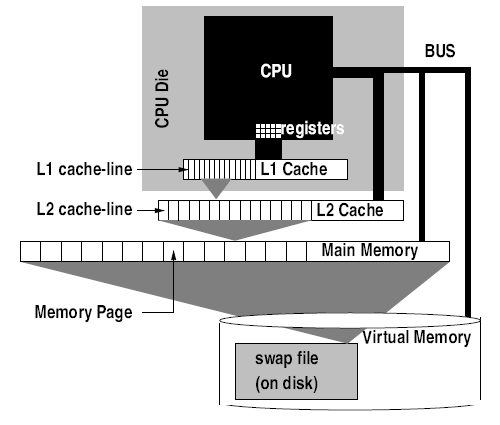
\includegraphics[width=0.4\textwidth]{./pictures/Fig1}
  \end{center}
  \caption{Hierarchical Memory System}
  \label{fig:fig1}
\end{wrapfigure}

Hard Disk drives are the cheaper, scalable and reliable solution for data storage but due to mechanical parts involved in the data access it has considerable latency issues as compared to other storage media and thus lies at the bottom of the storage hierarchy in terms of performance (Figure 1).

RAM or DRAM lies below high speed L1/L2 cache or SRAM but above any other storage medium in memory hierarchy system categorized as increase in performance from bottom to top as shown in figure 1. Since the SRAM cannot be extended in size due to hardware limitations therefore DRAM or RAM is the ideal candidate for data storage.


\begin{description}
  \item[Definition] As the name implies Main Memory Databases MMDB or In Memory Databases (IMDB) is a database management system which stores the complete database on physical memory or RAM. 
\end{description}

\subsection{History}
Most people argue in memory computing to be a relatively new and unproven technology. This is a myth rather than fact. For ages caching mechanisms is being used in traditional DRDBs which involves the most frequent use data inside RAM for fast access \cite{Mcobject-Myths} . In addition in-memory tables feature have also been part of some DBMS to hold data inside Main Memory. Also the use of DRDBs in main memory was a practice carried out to get better response times. 

This entails that MMDB are not new and considerable work has been done in this regard in 1980s. However they were not popular as the cost of memory and other limitations related to persistence of data were considered a problem. Many experimental MMDBs were developed then like MARS, HALO and MM-DBMS as part of research along with commercial systems like IBM Fastpath \cite{garcia1992main}. 

As of today IBM, Oracle and SAP being the top database vendors in the market have acquired the companies which were developing and marketing in memory database solutions \cite{pressRgiants}. Gartner\footnote{Gartner, Inc. is an American information technology research and advisory firm head-quartered in Stamford, Connecticut, United States} has placed In Memory computing as part of \emph{Top ten technology trends for 2013} \cite{gartner}. This clearly indicates the increase in the demand of MMDBs in market and their adaptation to the solutions in coming years.  

\subsection{Bounds of MMDBs}
MMDBs with their high performance mechanisms are the perfect contenders for embedded systems \cite{graves2002memory}. These systems with the evolution of smarter devices and expanding feature set needs to manage complex data structures which while written from ground up will require extra effort. With MMDBs pointer style low latency data access and simpler optimization techniques the embedded system developers have less things to worry about, stepping MMDBs adaptation to these types of systems. These systems include set-top boxes, network switches and consumer electronics. 

The real-time systems require time-critical access to and processing of massive amounts data. Example applications that handle large amounts of data and have stringent timing requirements include telephone switching, radar tracking and others. Furthermore as stated by \cite{ilprints39}, the real time database system design must not contain latency components like disk I/O operations, massage passing or garbage collection. Thus MMDBs architecture fits perfectly into the real-time application scenario. 

The role of the MMDBs has greatly expanded over the last couple of years as high-end 64-bit servers can now accommodate databases that are quite large – even terabytes in size. Therefore the applications for large IMDBs further include many popular large-scale Web applications and social networking sites. 

Nowadays, the data within an enterprise is distributed throughout a wide range of applications and stored in disjoint locations. Analytical reporting with amalgamated view on the data as a whole is a cumbersome and time-consuming process. Besides these reports are not entirely based on the operational data, but on combined data from a data warehouse by transforming it through ETL\footnote{ETL (Extract, Transform and Load) is a process in data warehousing responsible for pulling data out of the source systems and placing it into a data warehouse}process. Hasso has pointed out in \cite{plattner2011memory} that In-Memory data management assists the analytical operations resulting in planning, forecasting and faster decision making by separating it from operational data processing. Thus resulting in innovative and hybrid style of enterprise applications residing partially or fully in memory. 

% \subsection{Concurrency Control}  will discuss it later in the paper. Hammad 
% optimizer as well will be discussed later - hammad 
\section{Characteristics/Strong points of MMDB}
\begin{description}

\item[Pure In Memory Database]The differences between MMDB and traditional disk-based DBMS entails that DRDBs cannot be used as MMDBs and therefore a true In-Memory DBMS has to be written from bottom to top (Mcobject RealImmitation). The underlying goal of DRDBs is the minimizing of disk I/O even at the cost of CPU cycles in contrast to MMDBs goal for minimizing CPU cycles and Memory utilization. This implies that MMDBs can use the spared CPU cycles elsewhere to address durability and in some cases to create hybrid databases. 

\item[No Cache Maintenance] As already discussed in previous section, cache maintenance and management requires considerable resources which is eliminated in case of MMDBs. Cache synchronization and lookup processes adds to the function calls by processor and thus are expensive if aggregated together. MMDBs are indifferent to these mechanisms.

\item[Lightweight] Being lightweight is one of the common advantages IMDBs share and are helpful in embedded systems. This kind of databases is really simple: they don't implement any of the complex mechanisms used by traditional database to speed up the disk I/O therefore a small footprint.
Besides, as the data is readily available in memory and can be accessed by use of pointers, there is no need for storing redundant data in indexes (discussed later in data organization)

\item[High Performance] is another common feature for every IMDB, because they all store the whole database in main memory, avoiding disk access and minimizing CPU cycles and memory.

\item[Sound Memory Management ]Another key characteristic of Main Memory Databases are their sound memory management which derives that memory is a precious resource and needs to be looked after. This means that data alignment issues and sharing of heap memory through serialization be included in considerations for a MMDB memory manager as discussed in \cite{Mcobject-RealvsImmi}.

\item[New Breed of Application] MMDBs can be used as cache managers for large DBMS instead of being the primary database of application. This resulted in new breed of OLAP and OLTP applications which enables faster ETL processes and in-memory analytics.

\end{description}


\section{MMDB vs. DRDB : A Comparison}
In MMDBs, since the complete database physically resides inside Main Memory, a Main Memory Database Management System eliminates the most expensive Disk I/O operations which are the performance bottle neck in traditional DRDBs\footnote{Disk Resident Databases. Throughout this report we will use the terms “Disk-Resident”, “on-disk” and “disk-based” interchangeably to refer to traditional DBMSs that are “hard-wired” to store records to a file system on persistent media. While this media is usually a hard disk, it can also be a flash memory stick, solid state drive (SSD) or some other storage.}. Before delving deeper into variances it is pertinent to mention few important common questions and myths about MMDBs’.

\emph{Putting a DRDB in main memory will deliver us the same performance results as a MMDB} or \emph{MMDBs are the same traditional databases inside RAM}. This notion is not true at all. Although the traditional DRDB inside main memory out performs its instance on disk but while its comparison with pure MMDB the performance gap is far too much \cite{Mcobject-ramdisk}. Linux systems and now windows as well have the capability to create a RAM disk (File system inside the main memory). But a traditional DRDB deployed on such a virtually fast hard drive doesn't provide the same benefits of a pure MMDB. In-memory databases are less complex than their on disk counterparts fully deployed in physical memory and thus require minor usage of processing cycles and RAM.

Another popular feature which most database providers provide in their DBMSs are the creation of memory tables, through which certain tables can be designated for all-in-memory handling \cite{Mcobject-Myths}. So does this mean that \emph{with these memory features, DRDBs can compete with MMDBs performance?}. Not really as the problem remains the same as memory tables not only don't change the database design assumptions but also have certain additional restrictions. For example, in MySQL, memory tables cannot contain BLOB or TEXT columns and the maximum table size is fixed. Furthermore in contrast to MMDBs, the space that is freed up by deletion of tuples in an in-memory relation can only be used by the same relation, which is wastage of precious space inside RAM.

\emph{ IMDS Performance Can Be Obtained By Deploying a Traditional DBMS on a Solid-State Drive (Flash)}. Solid State Drives (SSDs) are nowadays another popular and widely used data storage devices in systems all over the world. Embedded and real time systems and even personal computers and laptops utilize their low latency data access features for specific applications. Since no moving part is included in SSDs, they outperform the hard disks in terms of disk I/O operations resulting in better responsiveness for database operations \cite{Mcobject-Myths} but other performance drains in the form of caching, disk I/O, data transfer etc will remain there. Moreover, even though these NAND based devices are faster and better in performance than hard disks but they are nowhere near to DRAMs amazing speeds \cite{ssds}. 

Comparing MMDBs with DRDBs we can find at least 4 key differences:

\begin{itemize}
\item Cache Maintenance
\item Data Transfer
\item Transaction Processing
\item Concurrency Control 
\end{itemize}

\subsection{Cache Maintenance}
Caching is a sophisticated mechanism that is used by all on disk traditional database management systems to improve performance due to high latency issues in hard disk. This incorporates the most accessed records to be placed inside main memory (database cache) for quick access. Sufficient overhead is involved in management of this mechanism which in case of MMDB is not required since all the data in readily available in RAM and can be accessed directly. Removal of caching logic removes the two expensive operations:

\begin{itemize}
\item Cache Synchronization : This ensures that database image in memory is synched with its physical contents on disk. Thus preventing the application to read inconsistent data. 

\item Cache lookup : is another process that determines if data that is requested by the application is in cache or not. If yes then it is fetched, otherwise a cache miss occurs and the corresponding page has to be read from the disk and load in memory. Furthermore it also takes responsibility and additional logic for protection of dirty data to be read by other applications before flushing it back to the disk after the transaction commits.
\end{itemize}


\subsection{Data Transfer}
Main performance degradation in DRDBs comes with the necessary file I/O operations that are performed on data as requested by the transactions from the application. This data undergoes extensive handling and unnecessary transfers before the application can use it as shown in \figurename{2a}. The chronological steps involved in the request can be summarized as follows by Graves in \cite{graves2002memory}:

\begin{figure}
	\centering
	\begin{subfigure}[b]{0.3\textwidth}
		\centering
		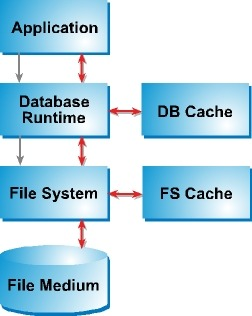
\includegraphics[width=\textwidth]{./pictures/fig3}
		\caption{On Disk Database}
		\label{fig:fig3a}
	\end{subfigure}
	\qquad \qquad
	\begin{subfigure}[b]{0.3\textwidth}
		\centering
		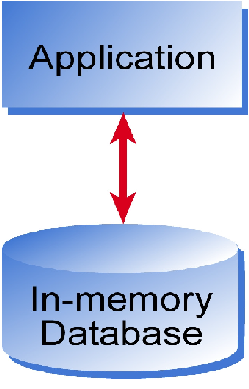
\includegraphics[width=0.5\textwidth]{./pictures/fig4}
		\caption{In-Memory Database}
		\label{fig:fig3b}
	\end{subfigure}
	\caption{Data Transfer}\label{fig:fig3}
\end{figure}

\begin{itemize}
\item application requests the data item from the database runtime through the database API.

\item The database runtime instructs the filesystem to retrieve the data from the physical media.

\item The filesystem makes a copy of the data for its cache and passes another copy to the database.

\item The database keeps one copy in its cache and passes another copy to the application.

\item The application modifies its copy and passes it back to the database through the database API.

\item The database runtime copies the modified data item back to database cache.

\item The copy in the database cache is eventually written to the filesystem, where it is updated in the filesystem cache.

\item Finally, the data is written back to the physical media.
\end{itemize}

In contrast the MMDB system entails little or no data transfer. The application may make copies of data in local variables but even this is not required as the MMDB system provides a direct pointer to the application, enabling it to deal with the data directly. Thus eliminating the multiple data transfer and streamlining processing . Besides cutting these extra copies saves memory and processor consumption and simplifies the design of MMDB systems. Data is copied directly from the IMDS to the application, and back from the application to the database, as shown in \figurename{2b}. Database API ensures that the data remains secure as the pointer is accessed through it. Moreover, in case of traditional databases, the cache flushed to disk require random access as data might be stored at different locations and thus adds up to the latency by disk seek, which in case of MMDBs is not a problem.
 
\subsection{Transaction Processing}
Transaction logging is a permanent feature of traditional on disk DBMS to ensure the ACID property of the database. We examine this memory-intensive processing in terms of atomicity and durability. 

\begin{description}
\item[Atomicity] In order to achieve atomicity, DRDBs use their hard-wired logging feature. The recovery process comprises of committing or rolling back transactions from log files. The IMDB should be able to handle the effects of unsuccessful transactions. In general terms, the problem has to explicitly with the data existent in the volatile memory, since all successful transaction are in a successful state only after been committed to the logging infrastructure. In order to comply with this transactional integrity, MMDBs use before and after-images of the database. When the application commits the transaction, the memory for before images are freed and are returned to memory pool. If it decides to abort due to any reason, the before-images are restored and newly inserted images are freed to be returned to the memory pool in a very fast and efficient way as compared to DRDBs.

\item[Durability] The logs are flushed to disk after transaction commits in DRDBs. The recovery process comprises of committing or rolling back transactions from log files in the event of a restart. In the event of a power or any other failure, the in-memory database image is lost forever as the memory is volatile and needs to be built again through some mechanism. This disadvantage of MMDBs suits most embedded systems like program guide application in set-top boxes which requires a connection to a satellite or cable head-end for downloading, a network switch that discovers network topology on startup, or a wireless access point that is provisioned by a server upstream. However in case of enterprise applications durability factor has to be addressed in an efficient way, as described later in this report, but it still contributes to performance degradation in MMDBs.
\end{description}

\subsection{Query Optimization}
Traditional on Disk Database query optimizer output results which aimed at minimizing the disk I/O operations while a MMDB query optimizer has a diverse goal for reducing CPU cycles and precious main memory. 

\section{Issues in MMDBs}
Although MMDBs are currently the new hype but before jumping on the bandwagon few issues and limitations needs to be discussed. There are methods which address almost all of these issues. Most in-memory database vendors provide the facility to the application developer to choose required quality over others depending upon the logic and need. 

\begin{description}
\item[Scalability]. 
According to Independent oracle users group data growth survey\cite{oracleDataGrowth}, the data growth of surveyed organizations is estimated around 25\% per year of their existing data. Is this a bad news for in-memory databases?.To overcome this problem there are two approaches
\begin{itemize}
\item Either get a better machine with more main memory or
\item Use distributed architecture by adding cheap commodity machines. 
\end{itemize}
Problem with first one is the cost involved with the new technology and second what is the guarantee that it will keep up with the growth rate? In case of distributed architecture, there are issues pertaining to the coordination and overhead between the nodes as well as the network latency but the system can scale indefinitely. A concept of RAMCloud as discussed in \cite{ousterhout2010caseRamClouds} is a viable solution but it comes with disadvantages of energy and space along with latency in cross-datacenters replication. However according to this paper, the failure of servers will be handled by the RAMCloud cluster within the recovery time objective of 1-2 seconds. 


\item {Durability \& High Availability}
As RAM is a volatile memory by design and in-memory databases keep the primary copy of records in Main Memory, all the stored data is lost whenever the system is powered off due to any reason. Therefore additional measures like check-pointing, shadow-pages along with logging needs to be built in to achieve durability. Similarly to achieve high availability, replication mechanisms on some persistent medium requires further implementation. These durability means are discussed later in this report. 

\item {Slow Start-up}
All durability and High Availability mechanisms, to an in-memory database system, make the database's startup terribly slow, because the database image is not stored on the hard disk, or on another persistent memory, and it needs to be reconstruct at every reboot, for example by reading the transaction log file and repeat all the operations executed before the power off. This issue can be mitigated by snapshots. But snapshot decreases performance of database once the system is executing the snapshot \cite{Mcobject-Myths}. Built-up of hybrid systems can also address this issue along with durability and High Availability. 

\item {Application Implementation}
As discussed in section 2 there are considerable differences between DRDB and pure In-Memory database, therefore the applications built for use with traditional DRDBs has to be modified to be used with an MMDB. This makes sense as the query optimization, memory management and the trade-off in performance by durability and high availability along with no disk I/O latency has to be taken into account while developing an application for MMDB. 

\item {Shared Memory for processing}
Main memory's primary usage lies with the processor for fast access and processing. This implies that it has to share the memory with the database and thus even the database API protects the data from being accessed but still the data is vulnerable to software errors. 

\end{description}



% IVAN: New content added from the new task split between our team mates:
% - My part begins with Indexing, this is not part of the data organization??, yes so I shall start with data organization.
% - Actually it is, because we have organized the structure as this document know explains, follow this document structure please.


\section{Data Organization}

In this section we will discuss the common data organization and access methods used by MMDBs. Relational Databases have been the backbone of business applications for more  than 20 years, trying to provide companies with a management information system for a set of applications. During all this time, we have dreamed with the possibility of having all the information at our fingertip, we even have sold this idea\cite{Plattner}.

\begin{wrapfigure}{R}{0.5\textwidth}
  \begin{center}
    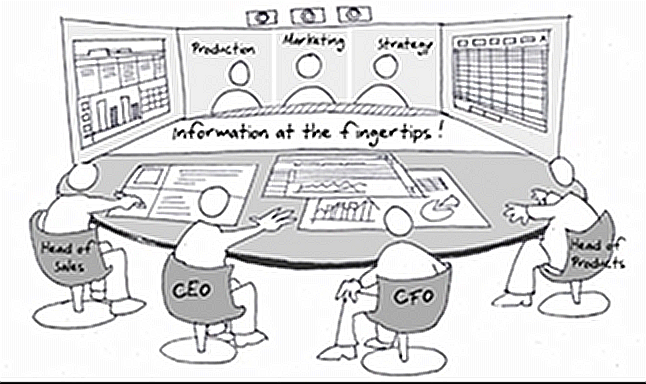
\includegraphics[width=0.4\textwidth]{./pictures/fig5}
  \end{center}
  \caption{Management of the Future}
  \label{fig:fig5}
\end{wrapfigure}

    But due to many reasons, we have not been able to offer this. And our systems have been separated in two main different groups: The online transaction processing (OLTP) and on line analytical processing (OLAP).

\subsection{OLTP and OLAP}
    % from \cite{Kemper}
    Under the OLTP classification, could be grouped systems with a high rate of day to day transactions, most of the database systems (as we know them) are mainly used for transaction processing. Some examples of OLTP systems are financial, sales, Manufacturing, order entry, banking transaction processing, human resources. All this systems performs relatively well mainly because they work on a small portion of the data. The TCP-C benchmark publish an average processing of 100.000 such sales transactions per second on a powerful system \cite{Kemper}.
    
    On the other hand, analytical, business intelligence and financial planning application were moved out to separated systems (for more flexibility and better performance). The OLAP Systems could be aimed toward specific task related to the company data warehousing. 
    
    Even though, this solutions are different in context, both are still based on \emph{ Relational theory } but with different technical approaches. The main purposes of this separation could be generalized into \emph{ performance } and maybe \emph{technical} issues. Even though both systems keep the essence in terms of relational theory, there are some important differences between them \cite{Plattner}.

    Moreover, recent development in the field of OLAP and the increased availability of main memory (sufficient enough to hold a completed compressed database) have enabled the processing of complex analytical requests in a fraction of a second and thus ease the development of new business processes and applications. The next step seems obviously to undo the separation between OLTP and OLAP and all requests be handled on a combined data set.

    %TODO: should I keep adding more info here? we can still talk about OLAP cubes, etc

    Now that the main memory is abundant, we have gone back to see the possibility of having a all-in-one MMDB. SAP\footnote{SAP AG: A German multinational software corporation that makes enterprise software to manage business operations and customer relations.} is one of the most enthusiastic companies pushing the use of Main Memory Databases for a mixed OLTP \& OLAP environment \cite{Plattner}, the company advertises SAP HANA as a generic MMDB solutions. 
    
    In this direction, it is suitable to estimate the challenges toward this join in technical perspectives, specifically, we have defined two main critical points related to data organization: The improved MMDB indexing system and the data Storage.

    
\subsection{MMDB Indexing}
It is mandatory to talk first about the differences between MMDB and on-disk DB, at first instance: In a MMDB Index, the main goal is to redesign the data structure and algorithm to make efficient use of \emph{ CPU } and \emph{ memory space } rather than minimize disk access, since we don't have disk of course. On the other hand, disk-oriented index structure are designed to minimize disk access and minimize disk space, this mainly because traditional database systems are CPU bounded because they spend considerable effort to avoid disk accesses.

A Main Memory oriented index structure is designed to reduce overall computation while using as little memory as possible \cite{lehman1986study}, since everything is in memory, MMDB Index could store only pointers to tuples or structures in the main memory (the actual data) instead of storing attribute values as on-disk DB usually does, decreasing efficiently the index footprint.

Although a MMDB system could be arranged in different ways, two main types of \emph{ Main Memory Index Structure } could be specified (Figure \ref{fig:fig6}): Order Preserving index structures and randomized \cite{lehman1986study}. Under the order preserving group could be summarized: arrays, AVL Trees, B Trees and T-Trees. T-Tree is one of the most important and well know structure, named T-Tree after its 'T' shape. On the other randomized group falls: Chained Bucket Hashing, Linear Hashing and Extendible Hashing.

\begin{wrapfigure}{R}{0.6\textwidth}
%  \begin{center}
  \vspace{-20pt}
    \centering
    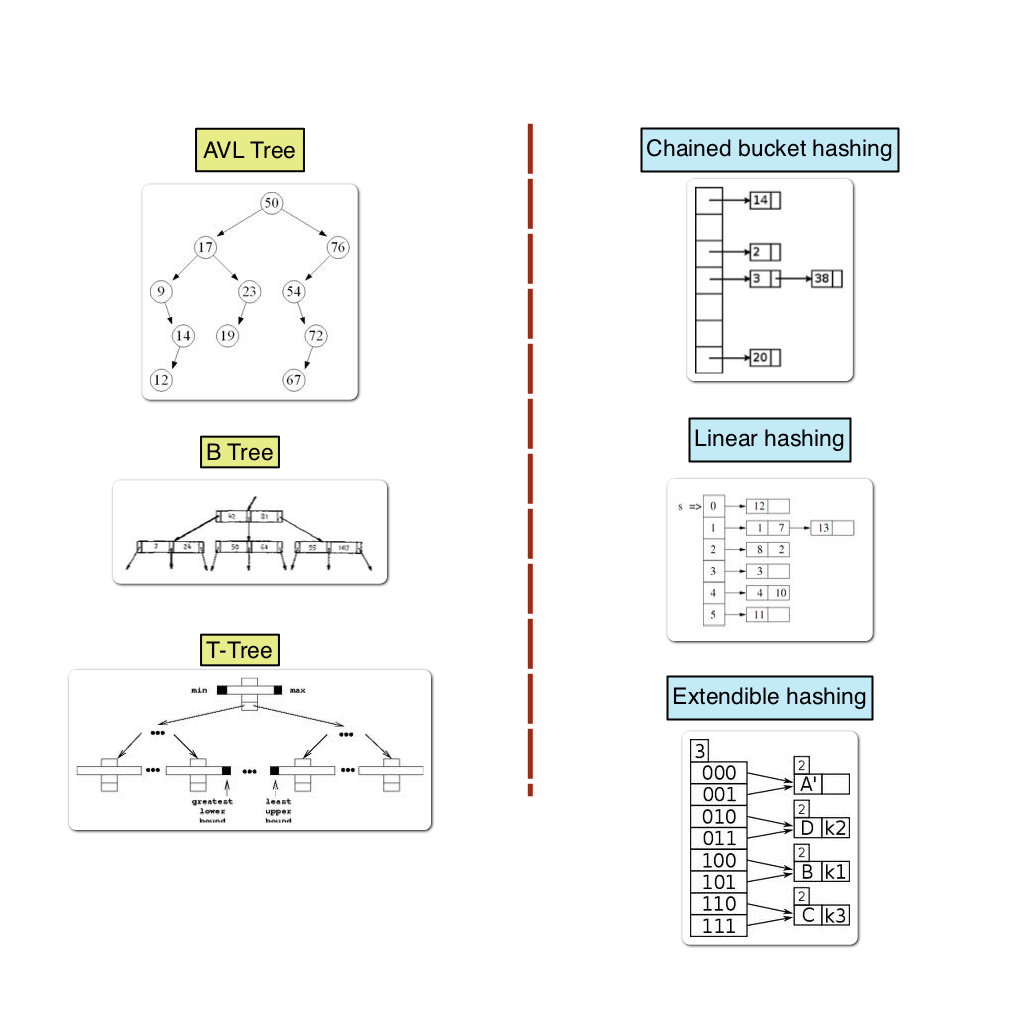
\includegraphics[width=0.4\textwidth]{./pictures/fig6}
%  \end{center}
  \caption{MMDB Index types}
  \label{fig:fig6}
  \vspace{-20pt}
\end{wrapfigure}


Although, the performance observed in a MMDB could be outstanding compared to a on disk DB, the index structure is a critical bottleneck \cite{leisadaptive}. The T-Tree (and one of the most developed) index technology involved in MMDB was proposed 25 years ago, and was designed based on the AVL and B Trees. Acording to \citeA{leisadaptive}, ``the dramatic processor architecture changes have rendered T-trees, like all traditional binary search trees, inefficient on modern hardware''.

TODO: maybe talk about details of t-trees\ldots 
% PV TODO: in lehman1986study there is more info about indexing and a detailed explanation of t-tree and its derived


\subsubsection{Column-Store Database System}

Column-oriented databases are based on vertical partitioning by columns, this is not a new idea, Column-oriented store where considered around 70s. The core of the functioning is based in the fact that each column is stored separately, having the logical scheme built around unique positioning keys \cite{krueger2011main}. This vertical data organization offers particular advantages to reading fewer attributes. According to \cite{Plattner}, in real world applications, ``only 10\% of the attributes of a single table are typically used in one SQL statement'', this could imply that: if during requests no unnecessary columns must be read, we could just use the columns independently of the related column attributes. Row oriented structures on hard drives normally can't perform this independence.

As a first premise, recent improvements in parallel processing of modern CPUs, could lead to think that a column oriented approach today seems to be ideal. The Column oriented storage has the following advantages: 

\begin{itemize}
  \item Column Store performs outstanding on modern CPUS.

  \item The Storage model is based on vertical fragmentation.

  \item Column Store Allow data compression

  \item Better memory consumption performance

  \item Data arranged in columns are better suited for parallel processing because of its independence.

\end{itemize}
   
Although, column oriented storage presents a lot of interesting features, it's worth to mention that there are also some drawbacks that kept this technology behind row oriented storage: for example: Column stores are expensive to update, but also having all data in main memory overcomes this limitation. Also column store increases seek time, but this is a concern only for on-disk DB systems.

From \cite{Plattner}, it seems that although more memory has been always useful, the database systems for OLTP where not well adopted in parallel environments, one of the reasons of this were problems like deadlocks and temporary locking in parallel transactions. So in general terms has not been a good idea. Really? review this since Plattner is one of the pro Column Oriented store.

Also from \cite{Plattner}, initial tests regarding in-memory databases using relational type based on \emph{ row storage } has not shown notable performance over RDBMSs. The opportunity for \emph{column based storage} now raises due the abundant availability of main memory. 

Compression is another characteristic that Column-oriented ease. The redundancy of column store and the homogeneous domain is an advantage and a convenience for compression techniques. All the data within a column belongs to the same type, and the entropy\footnote{The entropy could be defined as the similarities of data} is relatively low. 

TODO: talk more about column oriented, put some graphics

\section{Concurrency Control}
%multiversion concurrency control mechanisms 
The \emph{isolation} property of database ensures that the concurrent execution of transactions results in a system state that would be obtained if transactions were executed serially, i.e. one after the other. Providing isolation is the main goal of concurrency control mechanisms that are built within database systems while improving performance through concurrent execution. This isolation can be achieved through locking. \citeauthor{gray1993transaction} presented the two phase locking protocol \cite{gray1993transaction}, which states that for every read and write operation the transaction has to take locks (Phase-1) and then release them (phase-2) to ensure seralizability. Traditional DBMS use finer locks to reduce the lock contention which occurs due to concurrency. Since access to data in memory is almost instantly therefore the locks can be taken on larger granules, like at relation level, to perform the task quickly \cite{garcia1992main}. This ensures serializability and transactions will not be deadlocked. However in case of longer transactions this becomes the bottle neck of performance. Furthermore, these granularity levels can be varied dynamically to adjust to the conflicting transactions\cite{lehman1989concurrency}.


Multiversion concurrency control (MVCC) methods, being more robust and usually perform well, have been used for decades for variable workloads. These methods keep older versions of the objects alongwith timestamps and transaction IDs which acquire space. Since memory is precious therefore a variant of MVCC known as single version locking scheme suites best for main memory databases as discussed by \cite{larson2011high}. However in case of read only transactions this scheme underperform than other MV mechanisms as it has to acquire and release short read locks even for read-only transactions which impacts performance.


%multiversion concurrency control mechanisms 

\subsection{IMDB Data Recovery}

% PV: stupid idea: the memory comsumption is high since IDBM is memory based, but, OS Systems like Unix uses as much memory as they can in order to be more efficient, after coping all the memory, they start to swap and problems like trashing could happen.
% PV: stupid idea2: In a computer, all the memory has to be used because is already payed, the resource is there so take as much memory as you can.

%--------------------------------------------------------------------------------
% SAMAN part starts here:
%--------------------------------------------------------------------------------

\section{Recovery}

Since early 1980’s, that in memory databases gained attention; recovery is one of the main focuses of researches.  the characteristic of main memory database lets “master copies” or “working copies” of database be resident in memory. Main memory database requires a large amount of memory, but does not require the entire database to stored on the memory, it means in memory database systems still does the I/O process. ( a model of crash recovery ). Actually, it’s not applying the traditional concept of databases and technology that is applied to the traditional databases are not applicable to main memory databases. database recovery is among these technologies that we need to adapt it to the real time characteristic of databases. We need new algorithms and datastructures for in memory systems in order to improve system performance and efficiency. In this section we discuss or sometimes criticize the models of crash recovery that is introduced for main memory systems.

\subsection{Features of crash recovery in main memory databases}

We can divide the crash of database into three categories, the crash in transaction, system crash and media crash. Sometimes, the internal affairs of transaction many not reach the desired end; this type of crash is \emph{transaction crash} that results in leaving our database in an incorrect state. We do the \emph{ROLLBACK} to cure this problem, we cancel any modifications on the database by the transaction.

\emph{System crash} is another type of crash, it refers to any event that causes the system to stop and as a result to restart. Hardware errors, operating system crash, DBMS error  or a power cut may be the cause of this kind of crash. It may result in incorrect state in database and it needs to clear all changes to insure data consistency.

Third type of crash is \emph{media crash}. Also known as hard crash, this type of crash refers to external memory crash, such as disk crash, disk head impact and the instantaneous magnetic field interference. This kind of crash may damage part of our database and affect all the transactions that want to access this part of data. Basically, the possibility of this kind of crash is very smaller than transaction and system crash, but it is the most destructive of all.

When we consider Main Memory databases, the crash recovery and causes differ from traditional ones. it is mainly in following two aspects(A model of crash recovery):

\begin{enumerate}

  \item The main focus is on restoring the main memory. So, crash of transaction and system should be more emphasised. media crash is like traditional disk crash and the cure is like the traditional media crash recovery and may be easier in some scenarios.
  \item At backup step in recovery, we need to store data on our disk; so, it makes a bottleneck in efficiency of our transaction executing. Therefore, some traditional techniques may not be applicable and we need to think about some new algorithms and ideas.

\end{enumerate}


\subsection{A Model of Crash recovery by Tang Yanjun(todo: put a reference to article)}

In his crash recovery model, Tang Yanjun, proposes that each record has a unique object identifier (OID) that it’s value represent offset in virtual memory and also a dat file. The database achieve consistency by switching between two arrays index of zero and one that is created by OID. all the insert, update and delete operations should be done in this array. The other concept is shadow, which is shadow of OID array. It saves OID value recorded in database after the previous transaction submits. Moreover, he suggests tow indexed arrays in main memory database to record the characteristic of the object. one is current index and the other one is shadow index. It achieves consistency by storing double-index-structure. The current index points the to current data objects and the shadow index points to object in the database committed by the last transaction.

Therefore, when a crash in database occurs and database is in non-consistent state, it restores the database to the previous consistent state by executing the rollback operation. The illustration of Rollback operation is shown in figure n. When executing the Rollback, database copies the value of the shadow array to the current array.

System crash makes our database on the memory to clear so our database needs to restore and reinstall from a backup version on non-volatile storage. Yanjun proposes to recover the database using the double-index structure in the model.

Regarding media crash, the only solution that this model proposes is recovering the data from another disk backup files.

\subsubsection{Critic on the Yanjin model}

The model proposes to store the page tables on virtual memory, that at the first sight may seem good but it slows down our system. Although it made the assumption that the recovery model is for in memory databases but it didn’t take into the account that the virtual memory is much slower than main memory because it’s usually stored on disk or flash.

We can say that their model is good for ``Rollback'' but it should reside on the memory rather than virtual memory. But their model lacks the efficiency and performance that is needed for System crash backup and recovery. Their idea of storing each table on virtual memory would result in a lot of I/O process and as a result, decrease on speed and efficiency of the main memory database.

\subsection{A model of crash recovery by Li, Yang and Ye}

In their model, Li, Yang and Ye, propose a model of crash recovery for embedded main memory databases.  Their model has been applied in a real communication system ( Crash recovery, 2012). They introduced their model for SDR base station communication system but here we try to introduce the generalized model of their model.

The main memory database can be a relational database, and so the tables are relational. In these tables, there may be parent-child constraints between tables and the system should ensure the consistency of parent-child tables at any time. The new method that is proposed based on this, named flash recovery method.

They propose that we have a corresponding library for each table, each of these libraries have two directories. (figure of libraries and directories ).

The flash writing of the each domain is done to that domain’s library. For example, for  public domain, the data is written on the public library and in corresponding folders of “A” and “B” respectively. Moreover, there exist a “flash writing logo” to identify the progress. So, if a sudden crash happens when the system is running, the system will go to the correct flash directory to load data in order to ensure the data integrity after restart. You can see the flash writing and recovery proccess in figure a and b.

\subsubsection{Critic on the Li,Yang and Ye model}

In our opinion, in their paper they used checkpointing with another name and by duplicating the stored data they brought the RAID hardware system into software with less efficiency.

The main idea is to duplicate data, they do this in a sequential way and with control with software. backing up should be done in less time as possible to minimize the risk of system crash in the time of backup. When they do it in sequential way, it will oppose the system to the risk of crash.

if we say that the probability of crash in each second would be ($\alpha$) and the time that system is doing one backup is equal to t. then:\\

Probability that the system crashes when we do one backup on raid system:
\begin{equation}
 t*(\alpha) = (probability)
\end{equation}

Probability that the system crashes when we do two sequential backups:

\begin{equation}
 t*(\alpha)*2 = 2*(probability)
\end{equation}

So, the system is opposed to double probability of crash.

All in all, they haven’t gave a complete solution for a crash scenario and what they have gave can be implemented in more efficient way and with the minimized risk.

\subsection{ Discussion on recovery in database systems}



\section{Applications}

In-memory databases are most commonly used in applications that demand very fast data access, storage and manipulation, and also in systems that don’t typically have a disk but nevertheless must manage appreciable quantities of data.

An important use for in-memory database systems is in real-time embedded systems. IMDSs running on real-time operating systems provide the responsiveness needed in applications including IP network routing, telecom switching, and industrial control. IMDSs manage music databases in MP3 players and handle programming data in set-top boxes. In-memory databases’ typically small memory and CPU footprint make them ideal because most embedded systems are highly resource-constrained.

Non-embedded applications requiring exceptional performance are an important growth area for in-memory database systems. For example, algorithmic trading and other applications for financial markets use IMDSs to provide instant manipulation of data, in order to identify and leverage market opportunities. Some multi-user Web applications – such as e-commerce and social networking sites – use in-memory databases to cache portions of their back-end on-disk database systems. These enterprise-scale applications sometimes require very large in-memory data stores, and this need is met by 64-bit IMDS editions.(McObject Question and Answer about In-memory DBs)

\subsection{Growth of real-time Applications}

Network equipment manufacturers, telecom operators, securities exchanges and brokerages, airlines, shipping and logistics companies, and defense and intelligence agencies are examples of enterprises in which real-time applications are a necessity. The use of real-time processing to capture, analyze, and respond intelligently to key events is increasingly becoming the benchmark for corporate excellence.

For many companies, real-time applications aren’t elective—they are a necessity. Network equipment manufacturers, telecom operators, securities exchanges and brokerages, airlines, shipping and logistics companies, and defense and intelligence agencies are prime examples of enterprises that require real-time applications. In the past, building these applications also required the development of real-time infrastructure software. Fast but inflexible, these systems did the job as long as the applications remained static in their requirements. But dynamic industries quickly outpace static applications, and the cost to develop, test, and maintain  specialized infrastructure software is rarely justified when commercial alternatives exist.

With the growing speed of messages moving through business networks, the use of real-time processing to capture, analyze, and respond intelligently to key events is becoming the benchmark for corporate excellence. This isn’t important only for the execution and management of critical business processes. Customers expect highly tailored interactions and the utmost responsiveness from any company with which they do significant business.\\

Business activity monitoring, complex event processing, RFID/sensor-based applications, Web portals, and Web services are contributing to the movement of applications to the edge of the enterprise. Configured as dynamic collections of interrelated components, these applications are part of an overall approach known as a service-oriented architecture (SOA). However, most data sources still reside in the back office, dominated by large amounts of rarely touched legacy data surrounding smaller amounts of currently active information. A natural extension of SOA concepts includes lightweight, real-time data management in the application tier, connected to corporate data sources to provide real-time performance for currently active data. ( Extreme Performance Using Oracle Times Ten In-Memory Database)

\section{In Memory database solutions on market}
In recent years, a number of database vendors have marketed in-memory database solutions targeting different application developers. Some aim at real time embedded systems like McObject’s eXtreme DB \cite{Mcobject-RealvsImmi}. This versatile product is available in different flavors, each addressing a particular quality of traditional DBMS e.g. transaction logging edition, High Availability edition and hybrid Fusion edition which combines all the traditional DBMS properties with performance of a true in-memory database. eXtreme DB uses R-trees for geospatial data, Patricia tries for IP/telecom, KD-trees for multi-dimensional data and Query-by-Example (QBE), B-trees and hash indexes as access methods. 

The big database giant SAP has introduced its HANA database which is positioned as the core of the SAP HANA Appliance to support complex business analytical processes(OLAP) in combination with transactionally consistent operational workloads(OLTP) \cite{farber2012sap}. The in-memory computing engine allows HANA to process data stored in RAM as column and row stores according to the access patterns, allowing faster and better performance and aiding in decision making. 

Oracle is offering Times Ten as In-Memory database, which can be used as a preprocessing cache for its traditional flagship RDBMS or as a stand-alone database product. TimesTen uses Hash \& T-tree indices for data representation along with transactional logging and database checkpointing as a measure to provide durability \cite{oracleTimesTen}.

IBM has acquired SolidDB in 2008 and markets it as IMDB which maintains durability by keeping two separate but synchronized copies of database all the times as well as permanent log file stored on disk. It uses VTrie Indexes for Memory Tables and B+Tree for Disk tables. Recovery happens in less than one second through Hot Standby support \cite{IBMredbookSolidDB}. 

ALTIBASE HDB is an in-memory database that features a hybrid (memory plus disk) architecture. It is not open source, but it is free for non-commercial use and free for small business \cite{altibaseHDB}.

%-----------------------------------------------------------------
% IVAN: big table starting here
%-----------------------------------------------------------------
\begin{table}
\footnotesize
  \begin{center}
    %\begin{longtable}{|p{2cm}|p{2cm}p{2cm}p{2cm}p{2cm}p{2cm}|}
    \begin{tabular}{|p{2cm}|p{2cm}p{2cm}p{2cm}p{2cm}p{2cm}|}
      \hline
      & Times Ten & SAP HANA & eXtreme DB & IBM Solid DB & Altibase HDB \\
      \hline
      Data Organization
      &
      Hash \&; T tree
      &
      Row Store, Column Store
      &
      R-trees for geospatial data, Patricia tries for IP/telecom, KD-trees for multi-dimensional data and Query-by-Example (QBE), B-trees, hash indexes
      &
      VTrie Indexes for Memory tables and B+tree for Disk tables
      &
      Spatial Indexes \\
      \hline
      Recovery / Durability \& High Availability
      &
      Blocking \&; Fuzzy Check pointing with WAL logging Synchronous \&; Asynchronous Replication
      &
      WAL, shadow Paging and save points
      &
      synchronous (2-safe) and asynchronous (1-safe) replication, with automatic failover \&; Logging
      &
      Checkpointing, synchronous and asynchronous, Hot standby replication 
      &
      checkpointing and transaction logging. \\
      \hline
      Concurrency Control &Locks \&; latches with two isolation levels (Read Committed \&; Serialization)&MVCC in addition with a time-travel mechanism&MVCC&Pessimistic \&; optimistic concurrency control& MVCC \\
      \hline
      Support Hybrid&Yes&Yes&Yes&Yes&Yes \\
      \hline
      Cache support&Yes&Yes&Yes&Yes&Yes \\
      \hline
      OLAP Support
      &No&Yes&No&No&No \\
      \hline
      %\end{longtable}
      \end{tabular}
      \caption{Summary of MMDBs}
      \label{table:nonlin}
    \end{center}
  \end{table}
%--------------------- end table ------------------------
\normalsize



\section{Conclusions} 

% This is the point about conclusions and future directions (IVAN)
To Do: Conclusion regarding OLTP and OLAP merging, the bad news, what people says.

We could talk about: \emph{ MonetDB }, \emph{ VoltDB }??


%------------------------------------------------------------------------------------
%	BIBLIOGRAPHY
%------------------------------------------------------------------------------------
% This is the part about references

\bibliographystyle{apacite}
\bibliography{bibfile}
%------------------------------------------------------------------------------------
\end{document}
